\documentclass[conference]{IEEEtran}
\IEEEoverridecommandlockouts
% The preceding line is only needed to identify funding in the first footnote. If that is unneeded, please comment it out.
\usepackage{cite}
\usepackage{amsmath,amssymb,amsfonts}
\usepackage{algorithmic}
\usepackage{graphicx}
\usepackage{textcomp}
\usepackage{xcolor}
\def\BibTeX{{\rm B\kern-.05em{\sc i\kern-.025em b}\kern-.08em
    T\kern-.1667em\lower.7ex\hbox{E}\kern-.125emX}}
\begin{document}

\title{Administering Land Titles using Blockchain}

\author{
\IEEEauthorblockN{Tathagato Roy}
\IEEEauthorblockA{\textit{Roll No 2019111020}}
\and
\IEEEauthorblockN{Snehal Kumar}
\IEEEauthorblockA{\textit{Roll No 2019101003}}
\and
\IEEEauthorblockN{Rutvij Menavlikar}
\IEEEauthorblockA{\textit{Roll No 2019111032}}
}

\maketitle

\begin{abstract}
Blockchain technology has become a major disruptor in a lot of different sectors. While mainstream benefits till now have largely been constrained to economic and financial activities, recent developments have explored the use of Blockchain to solve larger societal problems. In this paper, we attempt to leverage Blockchain technology to digitise land ownership records and smoothen the overall process of land ownership verification and transfer of land deeds. We review and analyse the use of blockchain technology for administrating land titles. Importantly, we look at the preservation of titles as well as individual relationships to land through transfer of rights.
\end{abstract}

\section{Introduction}
\subsection{Problem}
Land titles document the ownership of land or immovable property.

The proper documentation of these records are of vital importance. The loss of land records pose a major cause of concern. Most countries use paper documents to store this data which is susceptible to manipulation, damage and permanent loss. In this paper, we propose a Blockchain based solution to address the issue of administering land titles.

\subsection{Motivation}

% Land title records are often inaccurate or defective due to administrative gaps. Because of these defects, inaccurate land titles misrepresent the actual nature of property rights being transferred in a transaction, creating a potential for subsequent losses. This adversely affects the use of land for activities like agriculture, housing, and industrial development. It also affects the use of land as collateral for credit. Title insurance helps protect land title holders (property owners) from the losses caused by such defects.

There exists widespread discrepancies, inaccuracies and outright falsifications in Land title records due to combination of administrative malfunction and corruption. These causes a cascading effect where all subsequent transactions on land based on faulty records becomes potentially faulty. This negatively impacts the use of lands in various economic activities like agriculture, housing and industrial development. Land is also often mortgaged for credit which is put at risk due to erroneous record keeping. Therefore Land Title Insurance are often utilised by land owners to protect themselves against losses caused by such defects.

Also, the transfer of ownership of a plot of land requires a lot of paperwork to be processed. At the rate paperwork in processed in government offices in India, it easily takes up to days for paperwork to be processed. And this processing also costs the government a lot in work force, work places and storage of papers.

\subsection{Beneficiaries}
\begin{itemize}
    \item Land Owners:\\Blockchain, being a distributed ledger technology ensures that as long as a user has their credentials, they can always generate authentic proof of ownership as and when required. This also eliminates the need for excessive paperwork, which takes days to process, and any trade of land can take place in a matter of minutes.
    \item Governing Authorities:\\In case of any disaster, the governing authorities can track any plot of land to it's current owner. Also, timestamped history of ownership for a plot of land can easily be stored and accessed. And eliminating paperwork can potentially reduce the operational costs drastically.
\end{itemize}

\subsection{Impact}
Land is one of the most important assets in any country. This has inadvertently also caused the most controversial and legal issues in the world. India has land disputes comprising of discourse over a land of 2.5 million hectares involving 7.7 million people, which contains a total of 66\% of all the pending court cases in India \cite{b3}. There have been many instances wherein bribes are paid to land registrars amounting to well over millions of dollars.

Recent natural disasters such as cyclones, floods which resulted in displacement of land caused many to lose their property after which the rightful owners could not be identified due to loss of data. This also meant that the victims could not claim any sort of compensation from the government also.

\section{Need of Blockchain} 
The currently existing system has many problems due to which there is a need of digitising the system with the inclusion of transparency and data reliability to avoid legal issues that arise. To this end, we believe that using blockchain is most suitable to make an efficient solution. Blockchain is a data structure on distributed ledger technology, which is concerned with capturing and transferring value. Also, with efficient and strong encryption, the authenticity of data is reliable.

\subsection{In absence of Blockchain why this may be complex?}
We emphasize on shifting to blockchain due to several issues found in the existing system.
\begin{itemize}
    \item Centralised storage of land records makes it vulnerable to natural or man-made disasters. Even in cases where the records are digitised, the failure of the central governing server can cause loss of all data.
    \item Traditional storage and database solutions are also vulnerable to manipulation by malicious and powerful entities.
    \item Traditional land record verification mechanisms are also found to be cumbersome, inefficient and costly.
    \item In a usual land transfer, although there are middlemen who assist in taking care of the details, their involvement adds additional complexity, delays, cost and the process no longer remains transparent.
\end{itemize}

\subsection{Advantages of Blockchain}
A successful implementation of the blockchain protocol would allow easy retrieval of the relevant data and smooth verification of ownership records, significantly improving the land owner's experience, reducing expenses and delay, greatly optimising the whole process. The other advantages of using blockchain in our system include:
\begin{enumerate}
    \item Robustness: It is robust to natural and man made disasters as damage of one or or more nodes in the network does not damage the overall functionality and security of the system.
    \item Error control: The nodes in the network ensure that the data is correct and valid before it is accepted and written in the block
    \item Security: By storing cryptographic hash of the previous blocks, it makes it extremely difficult for a powerful adversary to gain the necessary control to corrupt any previously entered data.
    \item Transparency: The inclusion of data in the blockchain makes the data and its management transparent to the public which adds credibility and trust in the system.
    \item Response Time: The protocols ensure that the response time for a service will be minimal, enhancing the customer experience.
\end{enumerate}

\section{Problem Statement}
Securing Property rights is an essential necessity for smooth functioning of any society. Land Rights is the most elemental part of Property Rights. In most developing nations and even in many developed nations these records are still stored as paper documents. Paper documents are vulnerable to being lost, destroyed or otherwise manipulated. Even in places where digitisation of land records have taken place, the transitions has not been seamless, i.e, there still remains a significant amount of unregistered land. Hence the process of verification land ownership remains a challenging and costly one. We propose a Blockchain based approach which aims to alleviate some of the challenges facing land ownership registration.

\section{Solution}
Blockchain is a distributed ledger that underlies the application and performs a few key functions that allow for an unprecedented level of security within the platform compared to all centralised platforms. The whole essence of Blockchain requires all members to be in a state of consensus, through a set of verification checks \& proofs that are calculated before every network change or transaction. We incorporate these functionalities of Blockchain with well defined and transparent procedures for it's functionalities.

We propose a Blockchain based approach which aims to alleviate some of the challenges facing land ownership registrations, and provides the following features:
\begin{itemize}
    \item Storage and easy access to ownership history
    \item Verifying authenticity of ownership
    \item Secure and fast transfer of ownership
    \item Decentralised and Immutable storage of transaction data with multiple copies
\end{itemize}

\subsection{Entities}
\begin{enumerate}
    \item \textbf{Land Owners:}\\They can register themselves on the blockchain as owners, validate their ownership using their credentials, and transfer their ownership to another person/organisation.
    \item \textbf{Buyers:}\\They can purchase land ownership from land owners registered in the system.
    \item \textbf{Government officials:}\\They have to verify land owners registering themselves in the system, verify the transaction of land ownership between two people/organisations, and can view time-stamped history of a land plot.
\end{enumerate}
The Land Owners and Buyers are not necessarily different roles in our system.

\subsection{Architecture}

We propose building a custom Blockchain which uses a PoA(Proof-of-Authority) protocol to build consensus. Proof of Authority is a variant of Proof of Stake which stakes the identity of the node instead. This assigns specific nodes as Validators whose function is to validate broadcasted transaction and add it to the Blockchain.

In our system the official government regulatory body will act as the validator nodes. Our system is parameterised by a integer $K$, where is $K$ is the number of signatures by validators needed to confirm the transaction before writing in the block. As one of the aim of our system is to provide guarantees in case a government worker is compromised due to corruption, blackmail or bribery, the parameter $K$ serves as proxy for the difficulty that a malicious adversary have to overcome in order to compromise the land ownership verification process. 

If at any point one of the validators suspect that the transaction is fraudulent, he/she can broadcast a flag which contains a message informing the network of the issues regarding the transaction. This message would be visible to all validators and can be used by them to decide to whether they should validate the transaction themselves. 

\begin{figure}[h]
\centering
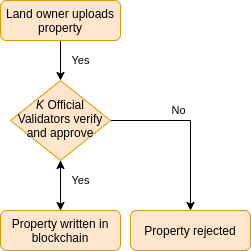
\includegraphics[width=0.3\textwidth]{LandRegister.png}
\begin{center}
    \tiny{Land Registration Flowchart}
\end{center}
\end{figure}

\begin{figure}[h]
\centering
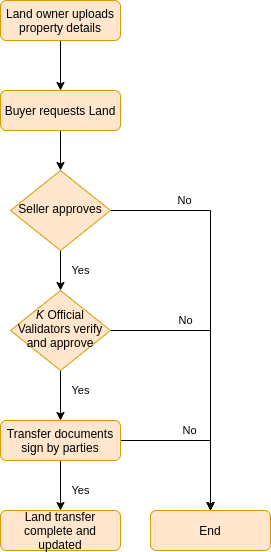
\includegraphics[width=0.3\textwidth]{LandTitle.png}
\begin{center}
    \tiny{Land Transfer Flowchart}
\end{center}
\end{figure}

The main ledger stores all the details corresponding to each property. It records the property transfer between buyer and seller and the subsequent change of ownership. It also allows for registration of land and assigns the land a unique id. This serves as an initial entry point for the land records (until now only recorded using paper deeds) to be entered into the system from which point on its ownership path through time can be reliably tracked using the blockchain ledger. 


\subsection{Suitable blockchain form}
To select the most appropriate form of blockchain, we used Wust and Gervais \cite{b1} and decided on \textit{Public Permissioned Blockchain}.

Public Permissioned is a form of Blockchain which allows anyone to read, but has an authorisation layer for granting writing privileges \cite{b2}. We used this form because of the following reasons:
\begin{enumerate}
    \item It ensures that only verified individuals can register, sell and buy land.
    \item It supports allocation of permission based roles for each node in the network.
    \item The public visibility of this form of Blockchain achieves transparency and promotes trust in the system among the members.
    \item It is lighter, faster and more energy efficient than its public counterparts.
\end{enumerate}

The central authority managing the network will be the Government land regulatory body.


\section{Analysis}
\subsection{Theoretical}
Blockchain has decentralised storage, and the ledger has multiple copies. So, if some of the servers storing some blocks were to be destroyed, even if one copy exists, the data can be retrieved.

The transaction ledger can and should be made publicly visible as per Section 4(1)(B) of the RTI Act and Public Records Act, 1993. And blockchain will make it easier to view the timestamped history of a land plot.

The data blocks in a blockchain being immutable, any unauthorised change in data can easily be detected and reverted. Hence, the authenticity and security of data is maintained.

The Proof-of-Authority protocol can help curb corruption and security threats in the following scenarios:
\begin{itemize}
    \item To authorise an illegal transfer of ownership, one would have to pay-off at least $K$ validators. Also, the validator's identities are made public. So if this transaction is caught in the future, the validators who authorised the transaction would be held responsible for it and this would lead to them losing their reputation in the network.
    \item In case any validator demands a bribe for their authorisation, any other validator can fill their place. And if this validator tries to block your transaction, they cannot hide their identity while doing so, and they would have to justify their actions.
    \item Since the identity is public, in case a hacker tries to impersonate as a validator, they will get exposed as well as they won't have sufficient authority to make any breaking damages.
\end{itemize}
Furthermore, using this protocol makes the system lightweight and energy efficient since it no longer requires use of mining type Proof-of-Work, rather it uses multiparty voting or signature scheme for consensus. Overall, this incentivises the nodes to act honestly as their best interest to maintain their reputation.

\subsection{Practical}
There are practical aspects of the system which need to be analysed before implementation to ensure the correctness.

\begin{itemize}
    \item Public Permission Blockchain: Gives an authorisation layer where a buyer or seller would require to upload a government issued ID to register themselves as an authorised participant in the network. This provides a somewhat weak form of security against use of false names or details for purposes of buying property, often done with criminal intent. This is also useful to differentiate the different roles (Government, Citizen) each type of nodes play in the network and what privileges each have while allocation.
    \item Data Integrity: Once an entry is made into the network, it can be reliably tracked through its transaction history. Hence, it is important to ensure the initial entry of ownership of land is correct, to maintain overall correctness. This is achieved by requiring that the initial request for registration of land be accompanied by submission of relevant documents to prove ownership of the land through the use of an online platform.
    \item Transactions: With the help of PoA and $K$ validators, we can be assured of the validity of the data and the response for the services to be met very quickly.
\end{itemize}

\subsection{Who will be bearing the cost of execution in blockchain environment?}
The management of the network and its subsequent cost will be taken care of by the government as it is done in a centralised system. For viewing any record, the gas required will also be taken care by the government in accordance with RTI. For each registration and transfer of property the customers will be required to pay a processing fee as a form of tax.

\subsection{If you want to productise, what are next steps?}
To deploy this system into production, we suggest using platforms like Quorum and Hyperledger Fabric which provide a public permissioned blockchain network that can be easily integrated in the system and managed by the government. 

\section{Future Work}
The proposed system addresses most of the problems faced by current traditional storage. There remains, however, the possibility of extending the current solution to other areas as well inclusion of features like:
\begin{itemize}
    \item The current system can be extended to include multiple ownership of the same land property. This will require some additional security protocols to maintain the integrity of the data.
    \item Lease and rental systems can be integrated in this system.
    \item Since most land properties are not bought directly but through the means of bank loans, the loan and investment system may be included within the network.
    \item Land asset can be liquidated by cryptocurrency by use of blockchain.
\end{itemize}

\section{Conclusion}
In this paper, we have highlighted the major concerns posed by current systems in land record management. Digitising this data makes the whole process more secure, robust and reliable. To solve this, we proposed a Blockchain based solution based on the requirements that needed to be resolved. Our architecture comprises of two types of entities, the land owners and the government management body, who interact with the system to ensure the validity and management of the data. We propose use of PoA protocol with identity as stake to make an incentive model for the body to act in the best interest of the network. And although this resolves the issues presented successfully, there remains additional features that can be added to the platform of land registry. 

\begin{thebibliography}{00}
\bibitem{b1} W{\"u}st, Karl and Gervais, Arthur, ``Do you need a blockchain?'' 2018 Crypto Valley Conference on Blockchain Technology (CVCBT), pp.45--54.

\bibitem{b2} ``Introduction To Permissioned Blockchains'', https://101blockchains.com/permissioned-blockchain/

\bibitem{b3} ``Access to justice survey'',
https://www.dakshindia.org/wp-content/uploads/2016/05/Daksh-access-to-justice-survey.pdf

\end{thebibliography}

\end{document}
